\begin{section}{Grafici ed immagini}
\begin{figure}[h]
	\centering
	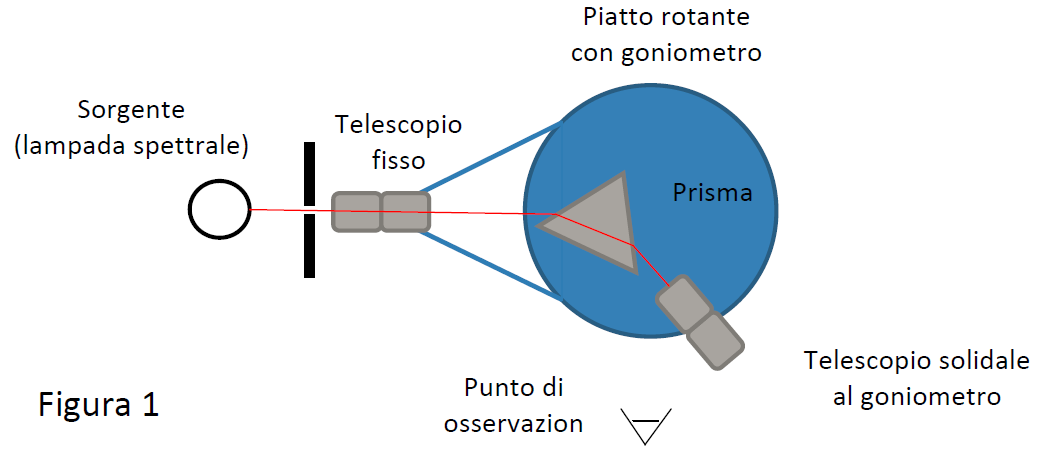
\includegraphics[scale=0.4]{spettroscopio_prisma.png}
	\caption{spettroscopio a prisma usato nella prima parte dell'esperienza}
	\label{f:spettroscopio_prisma}
\end{figure}

\begin{figure}[h]
	\centering
	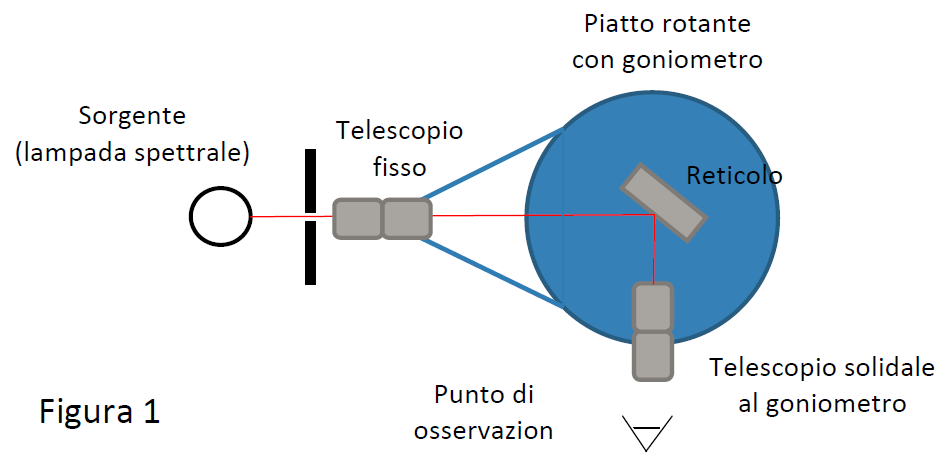
\includegraphics[scale=0.4]{spettroscopio_reticolo.png}
	\caption{spettroscopio a reticolo usato nella seconda parte dell'esperienza}
	\label{f:spettroscopio_reticolo}
\end{figure}


\begin{figure}[h]
	\centering
	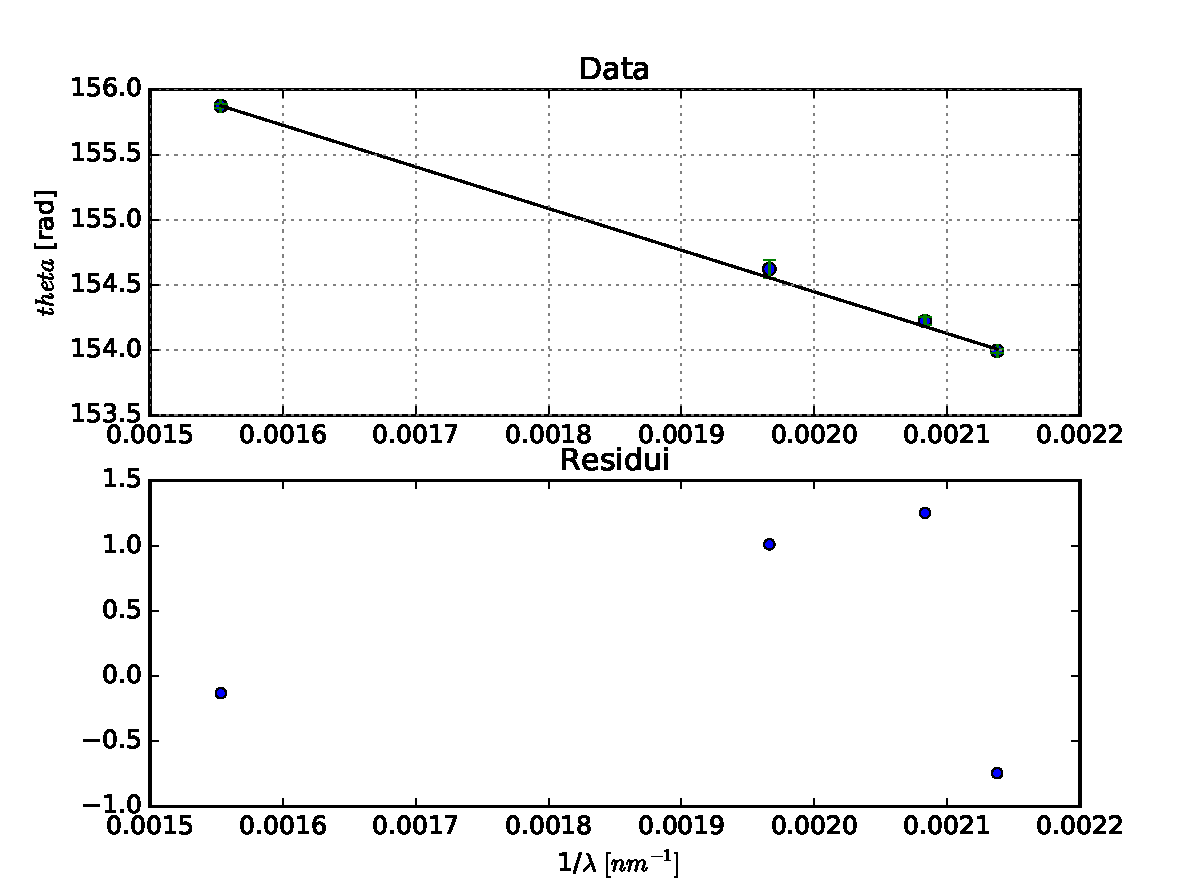
\includegraphics[scale=0.4]{calibrazione_sodio.pdf}
	\caption{calibrazione dello spettroscopio utilizzando la lampada a cadmio.}
	\label{f:calibrazione_cadmio}
\end{figure}


\begin{figure}[h]
	\centering
	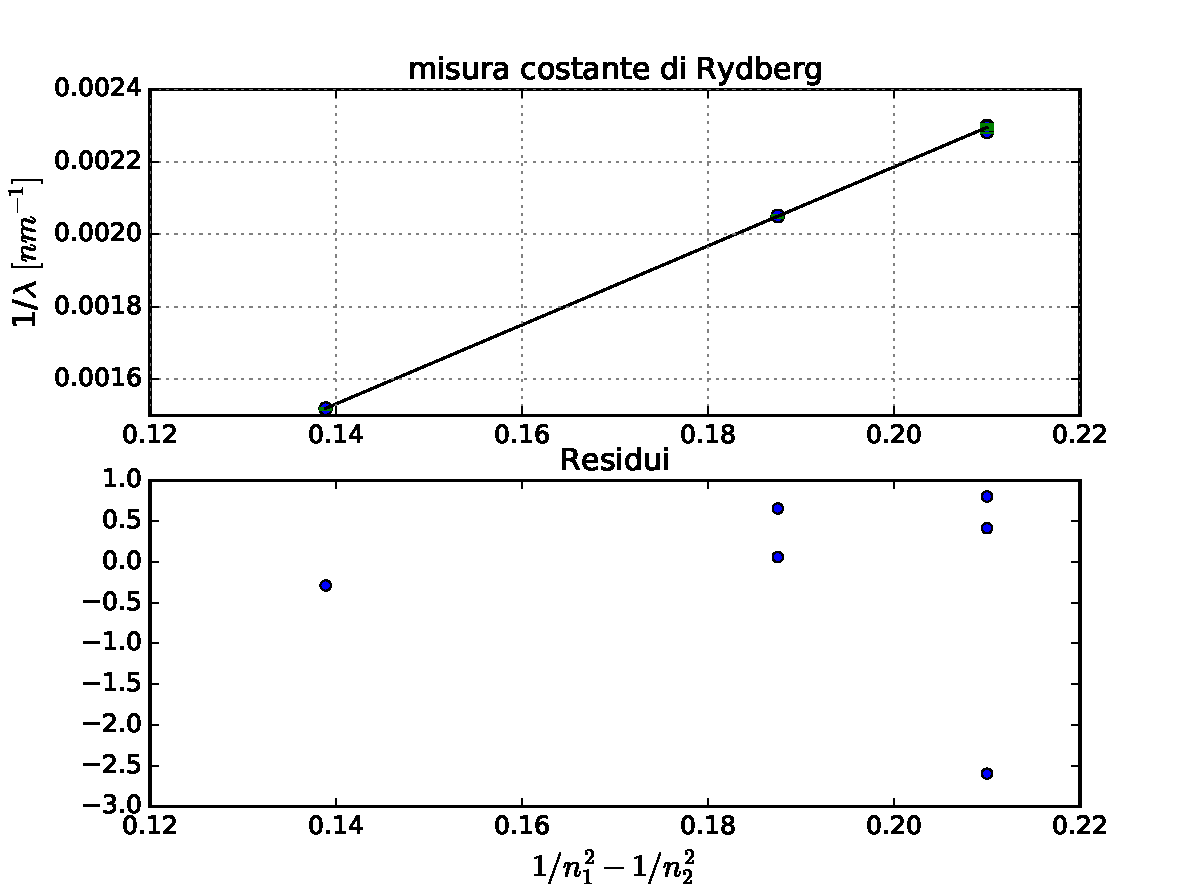
\includegraphics[scale=0.4]{rydberg.pdf}
	\caption{misura della costante di rydberg}
	\label{f:rydberg}
\end{figure}

\end{section}